Este documento tem como objetivo apresentar as atividades realizadas pelo bolsista André Luís Mendes Fakhoury no período de março de 2021 a setembro de 2021, referente ao projeto de Iniciação Científica com processo FAPESP de nº 2020/07224-5. O trabalho, intitulado ``Reconstrução de curvas por meio de características robustas extraídas de imagens'', é parte de umas das linhas de pesquisa do projeto temático FAPESP de nº 2019/07316-0, que visa a reconstrução de faces humanas a partir de informações reduzidas do domínio.

\section{O projeto e plano de trabalho}

O projeto de Iniciação Científica em questão está situado sob o contexto do mapeamento de características robustas entre espaços bidimensionais e tridimensionais. Este processo pode ser simplificado com a redução de informações a serem analisadas, como a representação de curvas a partir de um conjunto reduzido de pontos.

Para isso, serão analisadas principalmente curvas discretas extraídas de imagens. A partir destas curvas, pode-se analisar suas respectivas características robustas (também denominadas pontos importantes), que serão posteriormente responsáveis por reconstruir a curva original. Com isso, os seguintes objetivos específicos foram definidos para o projeto:

\begin{itemize}[noitemsep]
	\item Pré-processar as imagens com eliminação de ruídos, binarização e consequente segmentação;
	\item Extrair atributos de formas das imagens (contorno e cálculo da curvatura);
	\item Extrair características robustas em $\mathbb{R}^2$ para reconstrução de curvas com alta precisão a partir de imagens;
	\item Reconstruir as formas a partir das características robustas, por meio de curvas poligonais e operadores Laplacianos como sugerido por \citeonline{Sorkine2006};
	\item Aferir a qualidade da reconstrução a partir da curva original.
\end{itemize}

Para atingí-los, as seguintes atividades foram desenvolvidas: estudo das técnicas de reconstrução de curvas; pré-processamento de imagens; extração dos pontos importantes; implementação da reconstrução de curvas; avaliação e testes; combinação dos algoritmos.

O diagrama visto na figura \ref{fig:diagrama} descreve as principais etapas de desenvolvimento do projeto, e estas atividades foram dispostas no seguinte cronograma da tabela \ref{tab:cronograma} (atualizado conforme descrito no último relatório).

\begin{figure}[htb]
	\centering
	\caption{Diagrama de bloco das etapas de desenvolvimento}
	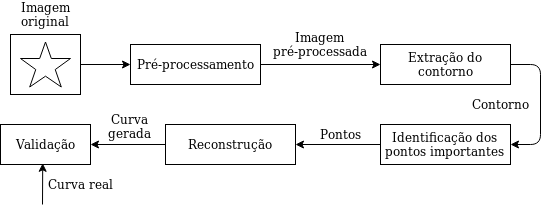
\includegraphics[width=.7\linewidth]{./img/diagrama.png}
	\legend{Fonte: Elaborada pelo autor.}
	\label{fig:diagrama}
\end{figure}

\begin{table}[htb]
	\footnotesize
	\centering
	\vspace{0.5em}
	\setlength{\tabcolsep}{0.05in}
	\begin{tabular}{|c|c|c|c|c|c|c|}
		\hline
		Atividades
		& \multicolumn{6}{c|}{Meses de trabalho} \\
		\cline{2-7}
		& 1\textordmasculine\ e 2\textordmasculine & 3\textordmasculine\  e 4\textordmasculine & 5\textordmasculine\  e 6\textordmasculine & 7\textordmasculine\  e 8\textordmasculine & 9\textordmasculine\  e 10\textordmasculine & 11\textordmasculine\  e 12\textordmasculine \\ \hline
		
		Estudo das técnicas de reconstrução de curvas  & $\bullet$ & $\bullet$ & & & &\\ \hline
		
		Pré-processamento & & $\bullet$ & $\bullet$ & & & \\ \hline
		
		Implementação da reconstrução de curvas & & $\bullet$ & $\bullet$ & & & \\ \hline
		
		Redação do relatório parcial & & & $\bullet$ & & & \\ \hline
		
		Extração dos pontos importantes & & & $\bullet$ & $\bullet$ & & \\ \hline
		
		Combinação dos algoritmos & & & & $\bullet$ & & \\ \hline
		
		Avaliação e testes & & & & & $\bullet$ & $\bullet$ \\ \hline
		
		Desenvolvimento do relatório final & & & & & & $\bullet$ \\ \hline
		
	\end{tabular}
	\caption{Cronograma de atividades para os 12 meses de trabalho.}
	\label{tab:cronograma}
\end{table}

As seguintes seções deste relatório descrevem com mais detalhes as atividades realizadas no projeto e outras considerações finais do aluno bolsista.